% Options for packages loaded elsewhere
\PassOptionsToPackage{unicode}{hyperref}
\PassOptionsToPackage{hyphens}{url}
%
\documentclass[
  english,
  man,floatsintext]{apa7}
\usepackage{amsmath,amssymb}
\usepackage{lmodern}
\usepackage{ifxetex,ifluatex}
\ifnum 0\ifxetex 1\fi\ifluatex 1\fi=0 % if pdftex
  \usepackage[T1]{fontenc}
  \usepackage[utf8]{inputenc}
  \usepackage{textcomp} % provide euro and other symbols
\else % if luatex or xetex
  \usepackage{unicode-math}
  \defaultfontfeatures{Scale=MatchLowercase}
  \defaultfontfeatures[\rmfamily]{Ligatures=TeX,Scale=1}
\fi
% Use upquote if available, for straight quotes in verbatim environments
\IfFileExists{upquote.sty}{\usepackage{upquote}}{}
\IfFileExists{microtype.sty}{% use microtype if available
  \usepackage[]{microtype}
  \UseMicrotypeSet[protrusion]{basicmath} % disable protrusion for tt fonts
}{}
\makeatletter
\@ifundefined{KOMAClassName}{% if non-KOMA class
  \IfFileExists{parskip.sty}{%
    \usepackage{parskip}
  }{% else
    \setlength{\parindent}{0pt}
    \setlength{\parskip}{6pt plus 2pt minus 1pt}}
}{% if KOMA class
  \KOMAoptions{parskip=half}}
\makeatother
\usepackage{xcolor}
\IfFileExists{xurl.sty}{\usepackage{xurl}}{} % add URL line breaks if available
\IfFileExists{bookmark.sty}{\usepackage{bookmark}}{\usepackage{hyperref}}
\hypersetup{
  pdftitle={Expecting to teach a novel golf putting task did not enhance retention performance: A replication attempt of Daou and colleagues (2016; 2016)},
  pdfauthor={Brad McKay1,2, Julia Hussien1, Michael J. Carter2, Zachary D. Yantha1, \& Diane M. Ste-Marie1},
  pdflang={en-EN},
  pdfkeywords={Motor learning; Pre-registered; Two-one-sided-tests; Sequential analysis},
  hidelinks,
  pdfcreator={LaTeX via pandoc}}
\urlstyle{same} % disable monospaced font for URLs
\usepackage{graphicx}
\makeatletter
\def\maxwidth{\ifdim\Gin@nat@width>\linewidth\linewidth\else\Gin@nat@width\fi}
\def\maxheight{\ifdim\Gin@nat@height>\textheight\textheight\else\Gin@nat@height\fi}
\makeatother
% Scale images if necessary, so that they will not overflow the page
% margins by default, and it is still possible to overwrite the defaults
% using explicit options in \includegraphics[width, height, ...]{}
\setkeys{Gin}{width=\maxwidth,height=\maxheight,keepaspectratio}
% Set default figure placement to htbp
\makeatletter
\def\fps@figure{htbp}
\makeatother
\setlength{\emergencystretch}{3em} % prevent overfull lines
\providecommand{\tightlist}{%
  \setlength{\itemsep}{0pt}\setlength{\parskip}{0pt}}
\setcounter{secnumdepth}{-\maxdimen} % remove section numbering
% Make \paragraph and \subparagraph free-standing
\ifx\paragraph\undefined\else
  \let\oldparagraph\paragraph
  \renewcommand{\paragraph}[1]{\oldparagraph{#1}\mbox{}}
\fi
\ifx\subparagraph\undefined\else
  \let\oldsubparagraph\subparagraph
  \renewcommand{\subparagraph}[1]{\oldsubparagraph{#1}\mbox{}}
\fi
% Manuscript styling
\usepackage{upgreek}
\captionsetup{font=singlespacing,justification=justified}

% Table formatting
\usepackage{longtable}
\usepackage{lscape}
% \usepackage[counterclockwise]{rotating}   % Landscape page setup for large tables
\usepackage{multirow}		% Table styling
\usepackage{tabularx}		% Control Column width
\usepackage[flushleft]{threeparttable}	% Allows for three part tables with a specified notes section
\usepackage{threeparttablex}            % Lets threeparttable work with longtable

% Create new environments so endfloat can handle them
% \newenvironment{ltable}
%   {\begin{landscape}\begin{center}\begin{threeparttable}}
%   {\end{threeparttable}\end{center}\end{landscape}}
\newenvironment{lltable}{\begin{landscape}\begin{center}\begin{ThreePartTable}}{\end{ThreePartTable}\end{center}\end{landscape}}

% Enables adjusting longtable caption width to table width
% Solution found at http://golatex.de/longtable-mit-caption-so-breit-wie-die-tabelle-t15767.html
\makeatletter
\newcommand\LastLTentrywidth{1em}
\newlength\longtablewidth
\setlength{\longtablewidth}{1in}
\newcommand{\getlongtablewidth}{\begingroup \ifcsname LT@\roman{LT@tables}\endcsname \global\longtablewidth=0pt \renewcommand{\LT@entry}[2]{\global\advance\longtablewidth by ##2\relax\gdef\LastLTentrywidth{##2}}\@nameuse{LT@\roman{LT@tables}} \fi \endgroup}

% \setlength{\parindent}{0.5in}
% \setlength{\parskip}{0pt plus 0pt minus 0pt}

% Overwrite redefinition of paragraph and subparagraph by the default LaTeX template
% See https://github.com/crsh/papaja/issues/292
\makeatletter
\renewcommand{\paragraph}{\@startsection{paragraph}{4}{\parindent}%
  {0\baselineskip \@plus 0.2ex \@minus 0.2ex}%
  {-1em}%
  {\normalfont\normalsize\bfseries\itshape\typesectitle}}

\renewcommand{\subparagraph}[1]{\@startsection{subparagraph}{5}{1em}%
  {0\baselineskip \@plus 0.2ex \@minus 0.2ex}%
  {-\z@\relax}%
  {\normalfont\normalsize\itshape\hspace{\parindent}{#1}\textit{\addperi}}{\relax}}
\makeatother

% \usepackage{etoolbox}
\makeatletter
\patchcmd{\HyOrg@maketitle}
  {\section{\normalfont\normalsize\abstractname}}
  {\section*{\normalfont\normalsize\abstractname}}
  {}{\typeout{Failed to patch abstract.}}
\patchcmd{\HyOrg@maketitle}
  {\section{\protect\normalfont{\@title}}}
  {\section*{\protect\normalfont{\@title}}}
  {}{\typeout{Failed to patch title.}}
\makeatother
\shorttitle{Expecting to teach replication}
\keywords{Motor learning; Pre-registered; Two-one-sided-tests; Sequential analysis}
\usepackage{lineno}

\linenumbers
\usepackage{csquotes}
\usepackage{pdflscape}
\usepackage{xcolor}
\raggedbottom
\ifxetex
  % Load polyglossia as late as possible: uses bidi with RTL langages (e.g. Hebrew, Arabic)
  \usepackage{polyglossia}
  \setmainlanguage[]{english}
\else
  \usepackage[main=english]{babel}
% get rid of language-specific shorthands (see #6817):
\let\LanguageShortHands\languageshorthands
\def\languageshorthands#1{}
\fi
\ifluatex
  \usepackage{selnolig}  % disable illegal ligatures
\fi
\newlength{\cslhangindent}
\setlength{\cslhangindent}{1.5em}
\newlength{\csllabelwidth}
\setlength{\csllabelwidth}{3em}
\newenvironment{CSLReferences}[2] % #1 hanging-ident, #2 entry spacing
 {% don't indent paragraphs
  \setlength{\parindent}{0pt}
  % turn on hanging indent if param 1 is 1
  \ifodd #1 \everypar{\setlength{\hangindent}{\cslhangindent}}\ignorespaces\fi
  % set entry spacing
  \ifnum #2 > 0
  \setlength{\parskip}{#2\baselineskip}
  \fi
 }%
 {}
\usepackage{calc}
\newcommand{\CSLBlock}[1]{#1\hfill\break}
\newcommand{\CSLLeftMargin}[1]{\parbox[t]{\csllabelwidth}{#1}}
\newcommand{\CSLRightInline}[1]{\parbox[t]{\linewidth - \csllabelwidth}{#1}\break}
\newcommand{\CSLIndent}[1]{\hspace{\cslhangindent}#1}

\title{Expecting to teach a novel golf putting task did not enhance retention performance: A replication attempt of Daou and colleagues (2016; 2016)}
\author{Brad McKay\textsuperscript{1,2}, Julia Hussien\textsuperscript{1}, Michael J. Carter\textsuperscript{2}, Zachary D. Yantha\textsuperscript{1}, \& Diane M. Ste-Marie\textsuperscript{1}}
\date{}


\authornote{

\begin{center}
\vspace{-2em} \textbf{\textcolor{red}{IN PRESS AT \emph{COMMUNICATIONS IN KINESIOLOGY}}}
\end{center}

Correspondence concerning this article should be addressed to Brad McKay, 1280 Main Street West, Ivor Wynne Centre Room AB-131 A1, McMaster University, Hamilton ON Canada, L8S 4K1. E-mail: \href{mailto:bradmckay8@gmail.com}{\nolinkurl{bradmckay8@gmail.com}}

\newpage

\addORCIDlink{Brad McKay}{0000-0002-7408-2323}

\addORCIDlink{Julia Hussien}{0000-0001-7434-228X}

\addORCIDlink{Michael J. Carter}{0000-0002-0675-4271}

\addORCIDlink{Zachary D. Yantha}{0000-0003-1851-7609}

\addORCIDlink{Diane M. Ste-Marie}{0000-0002-4574-9539}

Correspondence concerning this article should be addressed to Brad McKay. E-mail: \href{mailto:bradmckay8@gmail.com}{\nolinkurl{bradmckay8@gmail.com}}

}

\affiliation{\vspace{0.5cm}\textsuperscript{1} School of Human Kinetics, University of Ottawa\\\textsuperscript{2} Department of Kinesiology, McMaster University}

\abstract{
While research has identified several practice variables that purportedly enhance motor learning, recent replication failures highlight the importance of conducting high-powered, pre-registered replications. The ``expecting to teach'' phenomenon was first reported in the motor learning literature by Daou and colleagues and suggested learners benefit from practicing with the understanding they will later need to teach the skill. The extant data have been mixed but generally positive. While expecting to teach has been shown to enhance motor learning of a golf putt, the mechanisms linked with this benefit are yet to be determined. As such, this study sought to replicate the expecting to teach effect and to extend those findings by exploring participants' thought processes. Participants (N = 76) were randomly assigned to one of two groups in which they were told that they were learning a golf putt in order to 1) be tested on the skill or 2) to teach the skill to another individual. On Day 1, participants completed pre-test putts, a pre-acquisition intrinsic motivation inventory (IMI), a 2-minute study of an instructional booklet, 50 practice putts and a post-acquisition IMI. During practice, participants were also afforded opportunities to continue studying the booklet and to complete additional putts. Participants returned 24-hours later to complete a retention, a transfer (50 cm longer golf-putt), and a free recall test, as well as a post-study survey to reveal thoughts they engaged in after practice but before (or during) the retention test. Similar to Daou et al., no significant differences were found with study time, number of acquisition putts, or motivation. However, golf-putting performance during retention resulted in no differences for radial error, \(g = -.13\) (95\%CI {[}-.55, .29{]}), between the two groups and no differences were shown for the recall test. The present study fails to replicate the benefits reported in the original experiments.
}



\begin{document}
\maketitle

A primary objective of motor skill acquisition research is to determine practice variables that will show enduring effects on motor performance. Research in cognitive psychology provides some evidence that participants who study information and expect to later teach that information retain declarative knowledge more effectively than those expecting to be tested (e.g., Bargh \& Schul, 1980; Benware \& Deci, 1984; Nestojko et al., 2014), although some experiments have not found the same advantages (e.g., Ehly et al., 1987). Motivated by the findings of this literature, Daou and colleagues tested whether this expecting to teach effect would translate to motor tasks that require both procedural and declarative learning processes (Daou, Lohse, et al., 2016; Daou, Buchanan, et al., 2016). In their first two experiments to test the effect, participants attempting to learn to putt a golf ball were randomly assigned to two groups: One group was told that they would teach someone the next day on how to do the golf putt (Teach group) and the other was told they would be tested (Test group). In actuality, both groups were tested the next day.

The expecting to teach effect was evidenced at both procedural and declarative levels (Daou, Lohse, et al., 2016; Daou, Buchanan, et al., 2016). At the procedural level, the Teach group exhibited superior putting accuracy and precision during both retention and transfer tests (post-tests) over those expecting to be tested. Similarly, the Teach group showed superior declarative knowledge, as measured by free recall of golf putting information that had been in a study pamphlet, as compared to the Test group. Additionally, these two experiments included motivation and anxiety/pressure measures to determine whether the effects of expecting to teach were due to direct or indirect effects on motor performance. Indirect effects of motivation and pressure were ruled out due to no demonstrated differences in these measures between the two groups. Consequently, expecting to teach was described as directly enhancing motor learning.

With no reliable differences in affective-motivational mechanisms, possible contributions from information processing mechanisms were also examined. Daou, Lohse, et al. (2016) quantified the amount of time spent in motor preparation before each golf putt trial in acquisition and the Teach group yielded longer preparation times than the Test group. This preparation time difference, however, did not predict post-test accuracy or post-test precision when controlling for group; thus, only modest evidence was provided for possible information processing contributions. Further research by these authors have since replicated the expecting to teach effect for the Teach group, yet no differences were found between the two groups on varied electroencephalographic measures associated with motor preparatory processes (Daou et al., 2018). Such results have kept the understanding of the mechanisms for the expecting to teach effect uncertain.

Although Daou and colleagues have replicated the expecting to teach effect, they have shown that it may have limits, such as operating under low pressure situations, but not high pressure post-test situations (Daou, Hutchison, et al., 2019). Moreover, in recent experimentation, which used a 2x2 factorial design consisting of instruction set (Teach/Test) and motor preparation time (limited/unlimited), expecting to teach did not increase motor preparation time nor did it generate the motor learning advantages previously demonstrated (Daou, Rhoads, et al., 2019). A cumulative analysis within that paper suggested that the lack of an expecting to teach advantage may have been related to sampling variability. Further analyses on movement preparation time, however, suggested that motor preparatory processes were not a viable explanatory mechanism.

To date, the benefits for motor learning associated with expecting to teach has only been found in one research laboratory, and that laboratory has produced both significant expecting to teach effects (Daou et al., 2018, 2016; Daou, Hutchison, et al., 2019; Daou, Buchanan, et al., 2016) and null effects (Daou, Rhoads, et al., 2019; Rhoads et al., 2019). Lohse et al. (2016) have encouraged motor learning researchers to conduct replications stating that the replication of results in a different research laboratory greatly improves the precision of effect estimates (see also Open Science Collaboration (2015)). Given the simplicity of the expecting to teach intervention, its potential benefits, the previous support in the declarative domain, and the fact the evidence in the motor domain has thus far been limited to one research group, we felt a replication effort conducted in an independent laboratory was warranted. The primary purpose of this research was to replicate the findings of Daou and colleagues (Daou, Lohse, et al., 2016; Daou, Buchanan, et al., 2016)

Replications have been dichotomized into direct and conceptual categories (Makel et al., 2012). According to Makel et al. (2012) direct replications seek to duplicate the original methods as closely as possible, whereas conceptual replications follow similar methods, but researchers purposefully modify features of the experimental protocol to test the rigor of the underlying hypotheses. Within this dichotomy, the approach adopted here aligned more with that of a direct replication. That is, we adopted the methods of the original experiment which first showed the effect (Daou, Buchanan, et al., 2016), with the exception of including the more valid and reliable motivation and pressure measures that were used in their second experiment (Daou, Lohse, et al., 2016).

Beyond the direct replication, a secondary purpose was to explore other mechanisms that may be at play in the expecting to teach effect. Daou and colleagues had focused their efforts on possible affective-motivational mechanisms, as well as motor preparatory mechanisms that may occur during the acquisition phase (Daou, Hutchison, et al., 2019; Daou, Lohse, et al., 2016; Daou, Buchanan, et al., 2016). Throughout their series of experiments, however, there has been little support for either of these mechanisms. In the context of Kantak and Winstein (2012) motor memory framework, it is possible that the mechanism underlying the expecting to teach advantage is not at the encoding level (i.e., acting during the acquisition phase), but perhaps as a result of differences in consolidation or retrieval processes. Indeed Rhoads et al. (2019) suggested that their lack of replication of the expecting to teach effect may have been related to having their participants in the ``Teach'' groups immediately engage in the teaching experience after the acquisition phase. As a consequence, the ``expectation to teach'' was lifted during the 24 hour delay period before being tested; thus, diminishing offline consolidation processes that may have occurred in Daou and colleagues' preceding experiments. Other research has also shown that practice variables can impact consolidation processes in motor learning (Kantak et al., 2010; Kantak \& Winstein, 2012; Tanaka et al., 2010). There, however, appears to be little research, if any, that speaks directly to retrieval processes. To explore the possibility of contributions from consolidation and retrieval processes toward the expecting to teach benefits, participants were asked to complete a survey at the end of the experiment which queried about varied thought processes that were engaged in during two time intervals: (1) during the retention interval between the acquisition phase and post-test phase, thus considered to be tapping into consolidation processes, and (2) during the post-tests phase, thus considered to be aligned with retrieval processes.

Based on the results of Daou and colleagues (Daou, Lohse, et al., 2016; Daou, Buchanan, et al., 2016), the Teach group was anticipated to yield higher accuracy and precision scores in their golf putting as compared to the Test group. These procedural learning predictions would be supported by a significant main effect for Group (Teach, Test) on the combined scores of the delayed retention and transfer scores for both the radial error (accuracy) and bivariate variable error (precision) scores. Similarly, free recall performance was expected to be enhanced for the Teach as compared to the Test group on the declarative knowledge test, which would thus result in a significant main effect for Group.

\begingroup\fontsize{11}{13}\selectfont

\begin{landscape}
\begin{ThreePartTable}
\begin{TableNotes}
\item \textit{Note.} 
\item RH = Right-handed; LH = Left-handed; IMI = Intrinsic motivation inventory.
\end{TableNotes}
\begin{longtable}[l]{>{\raggedright\arraybackslash}p{13em}>{\raggedright\arraybackslash}p{20em}>{\raggedright\arraybackslash}p{20em}}
\caption{\label{tab:table1}Protocol modifications from Daou and colleagues and rationale for these changes.}\\
\toprule
Original protocol & Modification & Rationale\\
\midrule
Participants were RH and used RH putter. & Included LH and RH participants with the choice of using a LH or RH putter. A LH instructional booklet was made with adjusted images. & Given the large sample size required using both left-handed and right-handed participants was preferred.\\
\addlinespace
Instructions were read aloud from a script. & Instructions read aloud from a computer screen. & Multiple researchers involved in data collection so using a computer screen allowed for ease and consistency when communicating instructions.\\
\addlinespace
IMI administered at post-practice time point only & IMI administered not only at post-practice but also after pre-test putts. & Captured pre-test motivation to stay consistent with using covariate in analyses.\\
\addlinespace
Participant watched experimenter physically measure the shot error & Error measure via overhead camera and computer system. & Image capture was used mainly for ease of measurement.\\
\addlinespace
Auditory occlusion via ear plugs & Auditory occlusion via noise-cancelling headphones. & Better occlusion, more sanitary, and cost-effective.\\
\addlinespace
IMI and free recall were recorded via paper and pencil. & IMI and free recall were collected on a laptop. & Reduction of human error and ease of data entry directly into excel.\\
\addlinespace
Transfer test position created by moving target further away. & Transfer test position created by moving participant's starting position back. & Eliminated need for recalibration of the camera system for the transfer phase as the calibration occurs around the target location of the putt.\\
\addlinespace
No survey at completion of experiment. & Added a study extension survey at the end of the original protocol. & Opportunity to collect more information regarding the participants’ thought processes without impacting on original replication design.\\
\bottomrule
\insertTableNotes
\end{longtable}
\end{ThreePartTable}
\end{landscape}
\endgroup{}

\hypertarget{methods}{%
\section{Methods}\label{methods}}

We report how we determined our sample size, all data exclusions (if any), all manipulations, and all measures in the study (Simmons et al., 2012). This project was pre-registered using AsPredicted.org prior to beginning data collection and can be accessed here: \url{https://aspredicted.org/un9ap.pdf}. The methods used herein followed as closely as possible those of Daou and colleagues (Daou, Lohse, et al., 2016; Daou, Buchanan, et al., 2016); however, a few modifications were made to facilitate measurement and data collection procedures. Table \ref{tab:table1} presents the deviations taken from the original protocol and the rationale for these changes.

\hypertarget{missing-data}{%
\subsection{Missing Data}\label{missing-data}}

Unforeseen challenges were encountered during data collection which resulted in adopting changes from our pre-registered analysis plan. The putting surface used in this experiment was 66.04 cm wide at its narrowest point (the surface had a slight hourglass shape). Although only one putt left the putting surface during piloting and the first twenty-one participants in this experiment, the twenty-second participant putted seven pretest and six retention test putts off the surface (this participant has been excluded from all primary analyses). Once a ball left the putting surface it reached a tile floor that provided little resistance, resulting in the putts leaving the view of the camera and no data being recorded for the putts. Unfortunately, twenty-three of the subsequent participants putted at least one ball off the putting surface, and a total of 92 putts left the putting surface throughout this experiment. These putts were largely concentrated in the transfer phase (45 putts) and pre-test phases (34 putts). Since these putts could not be recorded, we have replaced them in the dataset with the maximum y-axis value for the participant in that phase as well as the maximum x-axis value possible. The sign of the x-axis error is unknown and was not recorded, which limits the reliability of our bivariate variable error analyses. We have given missing values the sign that is consistent with the participant's mean constant error for that block of trials. Given these limitations, we focus on retention test performance and radial error as our exclusive confirmatory analyses. The originally planned confirmatory analysis of radial error data combined across post-tests is still included as a secondary analysis. Further, a secondary analysis of retention test bivariate variable error is also provided. Additional deviations from our pre-registered analysis plan are included in Table \ref{tab:table2}.

\hypertarget{participants}{%
\subsection{Participants}\label{participants}}

Seventy-six university-aged adults (\(M_{age}= 20.74\) years, \(SD = 2.23\), 46 males, 30 females) with minimal experience golfing (\(M = 1.69\), \(SD = 5.43\) putting experiences in the past year) completed the experimental protocol. Based on Simonsohn (2015), target sample size was set \emph{a priori} to 140, representing 2.5 times the sample size \((N = 56)\) of Daou and colleagues' previous work (Daou, Lohse, et al., 2016; Daou, Buchanan, et al., 2016). The current sample size of 76 participants is the result of a number of factors. First, we planned to analyze the data using sequential analysis with two planned looks, one at \(N = 70\) and one at \(N = 140\) (Lakens et al., 2021). We used a Pocock adjustment to conserve an overall Type 1 error rate of 5\%; thus, setting the alpha at \(.029\) at each look. Once the sample reached \(N = 70\), the first analysis was conducted, and it was noted that the replication for procedural and declarative learning advantages, to this point, was not successful. As such, data collection resumed but, shortly thereafter, the COVID-19 pandemic occurred and human participant testing was no longer possible. In the hopes that testing could resume, we delayed further work on the project, but, regrettably, resumption has not been able to occur. Consequently, we are reporting the data on 76 participants.

All participants were naïve to the purpose of the experiment and were free of any motor or cognitive dysfunctions. Participants were informed that they would be entered into a raffle to win one of four \$20 gift cards to a location of their choosing. Prior to beginning data collection, all participants provided their informed consent in accordance with the institution's ethics board approved research protocol.

\begin{landscape}\begin{table}

\caption{\label{tab:table2}Justifications for deviations from our pre-registration.}
\fontsize{11}{13}\selectfont
\begin{threeparttable}
\begin{tabular}[t]{>{\raggedright\arraybackslash}p{14em}>{\raggedright\arraybackslash}p{16em}>{\raggedright\arraybackslash}p{25em}}
\toprule
Pre-registration & Deviation & Justification\\
\midrule
Total sample of N = 140. & Total sample of N = 76. & COVID-19 prevented continued data collection.\\
\addlinespace
Primary analysis combined retention and transfer tests in ANCOVA. & Only retention data were included. & Substantial number of putts went off the putting surface during transfer resulting in missing data.\\
\addlinespace
Primary analysis included BVE data. & BVE data were excluded from primary analysis but is still reported for retention and acquisition. & Putts that left the putting surface were missing from the dataset and would have influenced BVE data significantly.\\
\addlinespace
Exclusion based on outliers identified with MAD analysis. & Participant excluded due to excessive missing data. & Excessive missing data was unexpected, but exclusion seemed justified due to extent of the missing data.\\
\addlinespace
Exploratory independent t-tests of motivation data. & ANCOVA with pre-test included as a covariate. & Given that pre-test data are available for all motivation measures, ANCOVA is a more powerful analysis.\\
\addlinespace
Baseline data analyzed with independent t-tests & Not conducted & Upon further reflection, analyzing baseline data with inferential statistics was deemed unnecessary given that random assignment was used.\\
\bottomrule
\end{tabular}
\begin{tablenotes}
\item \textit{Note.} 
\item ANCOVA = Analysis of covariance
\item BVE = Bivariate variable error
\item MAD = Median absolute difference.
\end{tablenotes}
\end{threeparttable}
\end{table}
\end{landscape}

\hypertarget{task-and-materials}{%
\subsection{Task and Materials}\label{task-and-materials}}

The experimental task consisted of a short-distance golf putt on an artificial putting green (GS1018, JEF- World of Golf) using standard left- or right-handed blade putters and golf balls (Wilson Staff Fifty-Fifty). Data was collected entirely in a controlled laboratory environment and the task objective was to hit the ball such that it would land directly on top of a white target placed on the putting surface. At the end of the putting green, 132 cm from the participant, a foam lined backstop was set up to reduce unintentional auditory performance feedback in the event the golf ball rolled passed the surface of the putting green.

In order to score the putts, a FLIR Blackfly S USB3 camera (Model: BFS-U3-63S4C-C) fitted with an 8 mm fixed focal length Tamron lens (Model: LENS-80T4C) was mounted to a custom-made bracket anchored to a beam roughly 3.35 m above the putting green. The camera was plugged into a laptop in order to access a custom LabVIEW (National Instruments Inc.) program. The program was a modified version of the one developed by Neumann and Thomas (2008) that was adjusted to fit the experimental paradigm. In order to calibrate the camera system before and in between phases, a calibration board and string-line were used. Our custom program and camera system was used to measure all putts during the experiment and store the data (calculations and images) on the collection computer.

To evaluate the accuracy and consistency of the camera system, we took a sample of 40 putts (20 putts collected on two days a week apart) in which the ball was placed randomly from 0 to 125 cm in each of the four quadrants around the target (Neumann \& Thomas, 2008). Photographs were taken at each ball position and putts were scored using the camera system as well as by hand, which entailed measuring the distance from the centre of the ball to the target using a tape measure. We used the concordance correlation coefficient \((\rho_{c})\) (Lin, 1989) to compare the measurements of the camera system to hand measurements. The camera system was highly accurate \((C_{\beta} = .999)\) and consistent \((\rho_{c} = .998)\) as per the concordance correlation coefficient calculations (Lin, 1989).

Experimental instructions were presented using PowerPoint slide shows. Two golf-putting instruction manuals were used: Instructions for right-handed putting was provided by Daou and colleagues to be consistent with the original experiments being replicated, and the left-handed manual was duplicated by our laboratory to follow the right-handed manual exactly, with exception that images and instructions were for left-handed putting.

The Intrinsic Motivation Inventory (IMI) was used as a measure of intrinsic motivation (McAuley et al., 1989). The IMI consists of 24-items that provide data concerning participants' perceived interest/enjoyment, value/usefulness, effort/importance and pressure/tension experienced with the task. Responses were provided on a 7-point Likert scale ranging from 1-not true at all to 7-very true. Free recall of the information from the instruction manual was tested by asking participants to report, in as much detail as possible, any rules, methods or techniques that were used by them to execute the putt.

A survey was created on SurveyMonkey to tap into the thought processes that participants engaged in at two time points following the acquisition phase: 1) after the practice phase was over, but before the retention and transfer tests on putting performance began (i.e., during the retention interval), and 2) while executing the golf putts during the retention and transfer phase. The first timeframe was assumed to tap into possible activities that would assist with consolidation of the procedural and declarative information learned during acquisition, whereas the second was assumed to provide information concerning retrieval processes.

The first section of the survey checked, with a yes/no response, that the participants respected the instructions to not engage in overt activities to help them with the golf putt, such as continued practice or watching golf-putting videos and reading instructional information on golf-putting. The second section consisted of two questions that explored whether participants engaged in visualizing either themselves performing the golf-putt and/or images from the instruction booklet during the retention interval. They were to indicate yes or no, and if they responded yes, to estimate the amount of time engaged in visualization.

A third section, consisting of 17 items, was comprised of eight items that were reflective of content in the instruction manual, such as ``I thought about how my hands were placed on the putter'' or ``I thought about how my feet should be positioned hip width apart,'' thus they were identified as specific to the instruction booklet. Additionally, there were nine items that were self-generated by members of the research team that were not in the instruction manual, such as ``I thought about the path my ball would take'' or ``I thought about the force that I used to hit the ball to make a more accurate shot next time.'' We identified these as non-specific to the instruction booklet. This section was completed two times, each with a different instruction set prior to reading the items. These instruction sets were: 1) The next series of items are to get an understanding of some of your possible thought processes engaged in while putting today. Tick off any of those thought processes that you used, and 2) The next series of items are the same as those above, but now we would like to get an understanding of some of your possible thought processes engaged in after you finished putting yesterday to before you started putting today; this time interval does not include what you thought about during today's putting. Tick off any of those thought processes that you used, and for any that you did use, please give the approximate time in minutes and seconds for which you engaged in that thought process.

A final section began with participants queried as to whether they had any thoughts during the retention interval about what they would say to someone if they were going to teach someone how to golf putt. If they responded no, the last set of items did not appear. If they responded yes, the same 17 items appeared, and they were again asked to select any items they thought about and their respective durations. All items, however, were now worded to reflect the teaching aspect, for example ``I thought about how I would tell someone how to place their hands on the putter if I was teaching them how to golf putt'' or ``I thought about telling someone to think about the path the ball would take if I was teaching them how to golf putt.''

\hypertarget{procedure}{%
\subsection{Procedure}\label{procedure}}

\hypertarget{conceptualizing-the-replication-with-the-original-authors}{%
\subsubsection{Conceptualizing the replication with the original authors}\label{conceptualizing-the-replication-with-the-original-authors}}

Three of the authors of this paper met with the lead author of the original articles to gain clarification on procedural details to ensure proper replication. The lead author provided specific instructions, the instruction booklet, and other methodological details. As per Table 1, certain modifications, however, were adopted. The changes that were adopted were shared with three of the main authors of the original articles; all of whom agreed that the changes should not affect the ability to replicate. Prior to data collection and shortly after data collection started, two of the authors of the original articles visited the research laboratory at our institution and reaffirmed that the methodology was sound for a direct replication.

\hypertarget{experimental-protocol}{%
\subsubsection{Experimental protocol}\label{experimental-protocol}}

\textbf{Day 1.} Prior to the participant's arrival, the research assistant calibrated the camera image frame utilizing a string-line and calibration board. Upon arrival, participants completed the consent form and a demographic questionnaire that collected data on their age, gender, and golf putting experiences related to the past year and in their lifetime. Participants were then provided with both the left and right-handed putters and asked to choose which they would like to putt with. Once decided, they were informed of the handedness of their preferred putter and recorded that in the demographic questionnaire.

\textbf{Putting pre-test.} Participants were seated at a desk and guided through a laptop slide show that explained the pre-test instructions and were then led to the putting green where they were shown their starting point and target. Participants performed 10 trials with no feedback and then returned to their seated position. During the putting, they wore a blindfold and headphones to decrease sensory information that could be used as feedback. The experimenter returned the ball to the starting point each time and prior to each putt, the participant would lift the blindfold to locate the ball, re-position the blindfold so vision was occluded, and then immediately execute the putt.

\textbf{Pre-acquisition IMI.} Participants completed the IMI on a laptop computer in which the questions appeared in an excel file. Participants were instructed to read the item and to provide a number from 1 to 7 that reflected their level of agreement with the item, wherein 1 was anchored as not true at all and 7 was very true.

\textbf{Acquisition.} Participants were first guided through a slide show that provided them with instructions before their practice trials. The instructions for the two groups were differentiated by just one phrasing in the instructions: The Teach group were told ``you are trying to learn this golf putt because tomorrow you will \emph{teach someone how to do the task},'' whereas the Test group were told they were learning the golf putt because ``tomorrow you will \emph{be tested on how well you learned the task}.'' Next, participants were provided with the relevant instruction manual (i.e., the right-handed or left-handed version) face down and were instructed, once given the go-ahead, to study it for a minimum of two minutes, but they could do so for longer if they chose. Once they flipped over the manual, the study timer was started. After two minutes elapsed, they were asked if they wanted to continue studying the manual. If they stated they were done before the two-minute mark, they were encouraged to continue studying until the two-minutes were completed.

Once done studying, they were led to the putting green and reminded of their starting position and target. Unlike the pretest, they were not wearing the blindfold or headphones for any of the practice trials. All participants performed five blocks of 10 trials with one-minute rests between each block. During these rests, participants were seated at a table upon which the instruction manual was available, and they were informed that they could utilize the rest periods to continue to study the instruction manual. Time spent studying the manual was recorded manually by an experimenter and used to record total study time.

After the 50 golf putts, participants were informed that they had the option to perform up to 50 more trials (not organized in blocks) and/or to continue studying the manual, or to stop altogether. They were informed that, regardless of their decision, they would be required to stay in the laboratory until at least 45 minutes had elapsed from when they started studying the instruction manual. Additionally, participants were made aware that once they decided to stop practicing (putting or studying) they would not be permitted to start again. Once complete, the research assistant took note of the study time and then the participants were seated at the desk in front of the laptop.

\textbf{Post-acquisition IMI and instructions.} After the acquisition trials, participants responded to the identical 24-item IMI questionnaire as completed at pre-acquisition. Participants were then reminded of the time scheduled for their next day session which would be used for them to either teach someone the golf putt (Teach group) or be tested on their golf putting performance (Test group) depending on their group assignment. As well, participants were asked to refrain from ``practicing,'' which included watching golf putting videos, physically practicing, or reading golf putting instructions, prior to the next day session. Finally, participants were asked to provide their email if they wished to be entered into the raffle draw and were reminded to bring their cell phone for the next day's session in order to complete the mobile survey.

\textbf{Day 2.} Approximately 24-hours after completing their acquisition trials, participants returned for Day 2 testing. Upon arriving, participants in the Teach group were met with the statement ``I am so sorry, but the individual you were supposed to be teaching today has informed me that they cannot make today's session. We don't want the data we collected yesterday to go to waste, so instead, I am just going to test you on your golf putting. Are you OK with that?'' No one refused to be tested. Across both groups, in a randomized manner, the order of the retention and transfer test was counterbalanced.

\textbf{Retention and transfer.} Participants were seated and guided through a slideshow of the instructions for their first testing phase. They were informed that like the pretest, they would be performing 10 trials of their golf putt while wearing a blindfold and headphones. For retention, participants were informed that they would be performing the same putt as they did in the pretest and were shown their starting point and final target. For transfer, they were informed that although the target remained the same, the starting point had been moved back 50 cm. In both tests, participants were informed to keep their blindfold and headphones on between trials until the research assistant informed them their ball had been returned to the starting position. At that point, they could visually locate the ball and then return the blindfold into position.

\textbf{Free recall test.} Participants returned to the seated position at the table and were given access to an excel document on a laptop which instructed them to report, in as much detail as possible, any rules, methods, or techniques used to execute putts.

\textbf{Study survey.} Participants accessed a survey on the SurveyMonkey platform on their own mobile device and completed the survey while in the laboratory. Since the questions needed to be responded to while reflecting on critical time periods (i.e., during retention interval or during the post-tests) participants were asked to pay special attention to the instructions preceding each section. The first two sections required yes/no responses to the questions, and participants entered time engaged in visualization for items to which they responded with a yes. The final three sections involved participants using a checklist to indicate items they had thought about, either during the retention interval or the post-test golf putts. For those items selected, participants also entered an approximate time they had engaged in those thought processes.

\hypertarget{data-processing-and-analysis}{%
\subsection{Data processing and analysis}\label{data-processing-and-analysis}}

\hypertarget{sequential-analysis}{%
\subsubsection{Sequential analysis}\label{sequential-analysis}}

The \emph{a priori} analysis plan included two planned looks, one at \(N = 70\) and one at \(N =140\). The first look happened as planned and statistical significance was evaluated using the Pocock-adjusted alpha of \(.029\). The results at the first look were not significant. However, the planned total sample size could not be reached due to the onset of COVID-19, resulting in a final sample size of \(N = 76\). Therefore, the alpha for the final look needed to be recalculated based on the analysis that had occurred with \(N = 70\) and the actual final sample size. The first look took place with \(92.1\%\) (70/76 participants) of the total information that would be collected, and significance was evaluated with an alpha of \(.029\). Therefore, in order to maintain a \(5\%\) type 1 error rate, the adjusted final alpha was set to \(.0462\) (see Lakens et al. (2021) for a detailed tutorial on sequential analysis).

\hypertarget{physical-performance-data}{%
\subsubsection{Physical performance data}\label{physical-performance-data}}

Putting performance data were collected in two dimensions to facilitate measurement of precision in addition to radial error (Hancock et al., 1995). The putting target was located at the origin of the two-dimensional measurement grid with the coordinates \(0,0\). Radial error (RE), the two-dimensional equivalent of absolute error, was calculated for each putt using the Pythagorean theorem:
\[RE = (x^{2} + y^{2})^{\frac{1}{2}}\]
The two-dimensional equivalent of variable error, bivariate variable error (BVE), was calculated by taking the square root of the squared mean distance of each putt from the centroid (\emph{c}) of each block of \emph{k} putts:
\[\{(1/k)\sum_{i=1}^{k}[(x_{i} - x_{c})^{2} + (y_{i} - y_{c})^{2}]\}^{\frac{1}{2}}\]

Pre-test, retention, and transfer putting data (RE and BVE) were screened for outliers using the mean absolute deviation (MAD) technique with a pre-specified threshold of 3 to identify extreme cases. No outliers were identified so only one participant was removed due to too many missing trials.

\hypertarget{primary-confirmatory-analyses}{%
\subsubsection{Primary confirmatory analyses}\label{primary-confirmatory-analyses}}

The primary confirmatory analyses were conducted on retention test RE data by fitting an analysis of covariance (ANCOVA) with pre-test RE included as a covariate and group (Teach, Test) as a between-subjects factor.

\hypertarget{secondary-exploratory-analyses}{%
\subsubsection{Secondary Exploratory analyses}\label{secondary-exploratory-analyses}}

\textbf{Physical performance.} The originally planned primary analysis of radial error data was conducted by collapsing retention and transfer RE and fitting an ANCOVA with pre-test RE included as a covariate and group (Teach, Test) as a between-subjects factor. Due to excessive missing data during transfer, bivariate variable error data were only analyzed for the retention test. An ANCOVA was fit with pre-test BVE included as a covariate and group (Teach, Test) as a between-subjects factor.

Non-significant differences at retention were followed up by comparing the radial error results from the present experiment to a meta-analytic estimate of the original experiments reported by Daou and colleagues (Daou, Lohse, et al., 2016; Daou, Buchanan, et al., 2016). The authors of the original papers provided the data necessary to calculate effect sizes for input into a random effects meta-analysis. An equivalence test (Lakens, 2017) was conducted based on the lower bound of the 95\% confidence interval from the meta-analysis of original results.

Additional exploratory analyses of physical performance data were conducted on the acquisition RE and BVE data by fitting mixed 2 Group (Teach, Test) X 5 Block (Blocks 1-5) analysis of variance (ANOVA) models with repeated measures on the second factor. The number of additional putts practiced following the acquisition phase were analyzed via one-way ANOVA with Group (Teach, Test) as the between-subjects factor. Likewise, a similar one-way ANOVA was conducted on total time spent studying during the acquisition phase.

\textbf{IMI.} Individual scores were calculated by averaging the responses for items related to interest/enjoyment (7-items; pre-test \(\alpha = .88\), post-test \(\alpha = .92\)), value/usefulness (7-items; pre-test \(\alpha = .87\), post-test \(\alpha = .91\)), effort/importance (5-items; pre-test \(\alpha = .88\), post-test \(\alpha = .97\)) and pressure/tension (5-items; pre-test \(\alpha = .80\), post-test \(\alpha = .76\)) for both pre- and post-acquisition responses. For six of the 24 items, a reverse score was calculated, prior to averaging, by subtracting the participant's response from 8. Each subscale of the IMI was subjected to separate analyses of covariance (ANCOVAs) with IMI pre-test scores included as a covariate and Group (Teach, Test) as a between-subjects factor.

\textbf{Free recall.} Similar to Daou and colleagues (Daou, Lohse, et al., 2016; Daou, Buchanan, et al., 2016), participants each received four individual key concept scores (scored out of 1), and a total key concept score (scored out of 4). These key concepts were derived by the expert golfer who provided the initial putting instructions to Daou and colleagues and included 1) ``establish proper grip,'' 2) ``place the putter head behind the ball and take a hip-width stance,'' 3) ``place the eyes directly over the ball by hinging from the hips,'' and 4) ``stroke the ball without breaking the wrists.'' Points were calculated as 0 if the concept was not recalled, and 1 if it was recalled, except for key concepts 2 and 3 in which half points were awarded if the participant mentioned one of the two statements.

\textbf{Survey.} The number of participants that responded positively to the use of visualization and thoughts engaged in related to teaching the golf putting skill were recorded. Descriptive statistics were calculated for the relevant sections of the survey, which included: 1) from section 2, the time spent engaging in visualization during the retention interval (i.e., interval of time post-acquisition trials and post-test phase), 2) from section 3a the number of thoughts selected during the post-test phase, 3) from section 3b, the number of thoughts selected and the time spent engaging in those thoughts during the retention interval, and 4) from participants who responded `Yes' in section 4, the number of thoughts selected and the time spent engaging in those thoughts during the retention interval.

\hypertarget{results}{%
\section{Results}\label{results}}

Results from the final sample are reported below. Data, analysis scripts, and results from the interim analysis can be accessed here: \url{https://osf.io/r6z84/}. After removing one participant due to missing data, the resulting sample included 42 participants in the Test group and 33 participants in the Teach group.

\hypertarget{confirmatory-analyses}{%
\subsection{Confirmatory analyses}\label{confirmatory-analyses}}

\hypertarget{retention}{%
\subsubsection{Retention}\label{retention}}

The Teach (\(M = 60.16\) cm, \(SD = 33.05\)) and Test (\(M = 57.89\) cm, \(SD = 26.94\)) groups were not significantly different at retention, \(F(1,73) = 0.383, p = 0.538\) (see Figure \ref{fig:fig1}). Pre-test accounted for a significant proportion of variance in retention performance, \(F(1,73) = 11.01\), \(p = 0.001\), \(R^{2} = .14\).



\hypertarget{secondary-analyses}{%
\subsection{Secondary analyses}\label{secondary-analyses}}

\hypertarget{original-primary-analysis}{%
\subsubsection{Original primary analysis}\label{original-primary-analysis}}

\textbf{RE.} The Teach (\(M = 68.26\) cm, \(SD = 31.32\)) and Test (\(M = 67.58\) cm, \(SD = 25.29\)) groups were not significantly different on the combined retention and transfer post-test, \(F(1,73) = 0.15\), \(p = 0.698\) (see Figure \ref{fig:fig1}). Pre-test accounted for a significant proportion of variance in post-test performance, \(F(1,73) = 11.58\), \(p = 0.002\), \(R^{2} = .12\).

\textbf{Retention BVE.} The Teach (\(M = 33.56\) cm, \(SD = 13.64\)) and Test (\(M = 37.44\) cm, \(SD = 13.17\)) groups did not differ significantly at retention, \(F(1,73) = 1.48\), \(p = 0.228\). Pre-test accounted for a non-significant proportion of the variance in retention, \(F(1, 73) = .44\), \(p = 0.508\), \(R^{2} = .007\).

\begin{figure}

{\centering 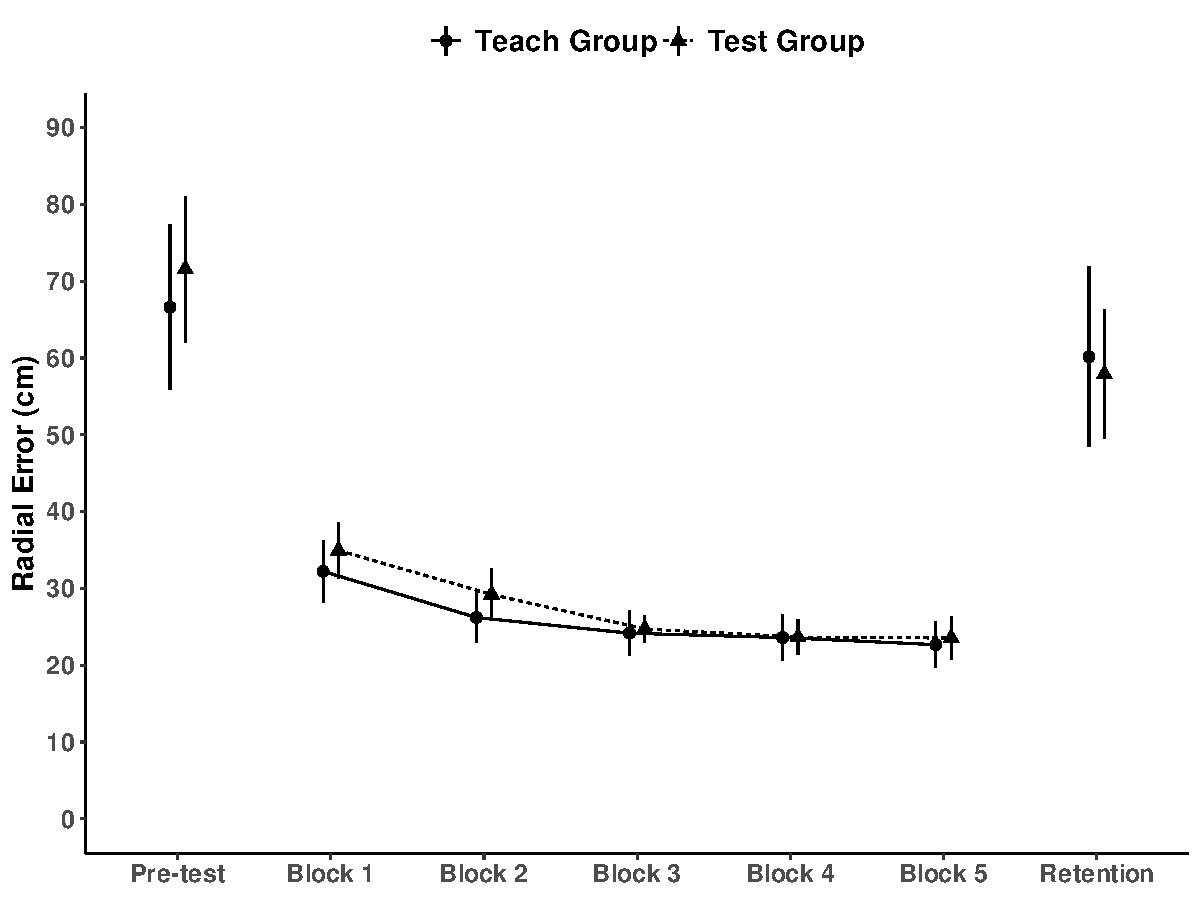
\includegraphics[width=1\linewidth,height=1\textheight]{../../figs/fig1} 

}

\caption{Mean radial error for both groups during the pre-test, acquisition, and transfer phases of the experiment.}\label{fig:fig1}
\end{figure}

\hypertarget{equivalence-test}{%
\subsubsection{Equivalence test}\label{equivalence-test}}

\textbf{Meta-analysis of original results.} Effect sizes (Hedges' \(g\)) from the original experiments (Daou, Lohse, et al., 2016; Daou, Buchanan, et al., 2016) were calculated with data provided by a senior author of the papers. Both experiments observed similar benefits for expecting to teach relative to test, as measured by radial error on retention test performance while controlling for pre-test radial error, \(g = 1.08\), \(95\%CI \,[.53, 1.63]\) (Daou, Buchanan, et al., 2016), \(g = .82\), \(95\%CI \,[.33, 1.3]\) (Daou, Lohse, et al., 2016). The random effects estimate based on these two experiments was \(g = .93\), \(95\%CI \,[.57, 1.29]\).

\textbf{Two one-sided tests.} Two one-sided tests (TOST) were conducted with equivalence bounds of \(.57\) and \(-.57\), based on the lower bound of the meta-analytic estimate above. The effect of expecting to teach on post-test radial error was significantly smaller than the lower bound estimate of the original experiments, \(g = -.02\), \(t(61.13) = 2.74\), \(p = .004\). The observed effect was in the opposite direction as the hypothesis, but was significantly larger than the negative equivalence bound, \(t(61.13) = -2.10\), \(p = .020\).

\hypertarget{acquisition}{%
\subsubsection{Acquisition}\label{acquisition}}

\textbf{RE.} The Huynh-Feldt correction was applied due to significant violation of the sphericity assumption. The Teach and Test groups were not significantly different at acquisition, \(F(1,74) = 0.78\), \(p = .380\). Both groups reduced their error over the course of acquisition, evidenced by a significant effect of block, \(F(3.48, 257.64) = 40.629\), \(p < .001\). The Group X Block interaction was not statistically significant, \(F(3.48, 257.64) = .948\), \(p =.428\) (see Figure \ref{fig:fig1}).

\textbf{BVE.} The Hyunh-Feldt correction was applied due to significant violation of the sphericity assumption. The Teach and Test groups did not differ significantly during acquisition, \(F(1,74) = 1.55\), \(p = .217\). Both groups significantly improved their precision over the course of acquisition, \(F(3.6, 266.61) = 27.33\), \(p < .001\).The Group X Block interaction was not significant, \(F(3.6, 266.61) = .65\), \(p = .611\).

\hypertarget{additional-practice-trials-and-study-time}{%
\subsubsection{Additional practice trials and study time}\label{additional-practice-trials-and-study-time}}

The Teach (\(M = 21.29\), \(SD = 18.95\)) and Test (\(M = 21.67\), \(SD = 21.24\)) groups did not engage in a significantly different number of free-choice practice trials following the acquisition phase of the experiment, \(F(1,75) = .14\), \(p = 0.708\). Similarly, the Teach (\(M = 130.30\) sec, \(SD = 58.74\)) and Test (\(M = 157.89\) sec, \(SD = 73.74\)) groups did not differ significantly in the amount of time spent studying the instruction manual, \(F(1, 75) = 3.12\), \(p = .082\).

\textbf{Free recall.} The Teach (\(M = 1.81\), \(SD = 0.97\)) and Test (\(M = 1.35\), \(SD = 1.06\)) groups did not differ significantly in the number of key concepts recalled, \(F(1, 72) = 3.80\), \(p = .055\).

\hypertarget{motivation}{%
\subsubsection{Motivation}\label{motivation}}

\textbf{Interest/enjoyment.} The Teach (\(M = 5.43\), \(SD = 1.11\)) and Test (\(M = 5.18\), \(SD = 1.34\)) groups did not differ significantly on the interest/enjoyment subset of the IMI, \(F(1, 74) = 0.02\), \(p = 0.88\). Pre-test accounted for a significant proportion of the variance in post-test interest/enjoyment, \(F(1,74) = 58.69\), \(p < .001\), \(R^{2} = .45\).

\textbf{Value/Usefulness.} The Teach (\(M = 5.15\), \(SD = 1.27\)) and Test (\(M = 4.64\), \(SD = 1.33\)) groups did not differ significantly on the value/usefulness subset of the IMI, \(F(1,74) = .18\), \(p = 0.67\). Pre-test accounted for a significant proportion of the variance in post-test value/usefulness, \(F(1,74) = 72.69\), \(p < .001\), \(R^{2} = .52\).

\textbf{Effort/importance.} The Teach (\(M = 5.54\), \(SD = 1.21\)) and Test (\(M = 5.0\), \(SD = 1.38\)) groups did not differ significantly on the effort/importance subset of the IMI, \(F(1,74) = 2.90\), \(p = 0.093\). Pre-test accounted for a significant proportion of the variance in post-test value/usefulness, \(F(1,74) = 85.73\), \(p < .001\), \(R^{2} = .54\).

\textbf{Pressure/tension.} The Teach (\(M = 2.20\), \(SD = 1.21\)) and Test (\(M = 2.39\), \(SD = 1.04\)) groups did not differ significantly on the pressure/tension subset of the IMI, \(F(1,74) = 2.45\), \(p = 0.123\). Pre-test accounted for a significant proportion of the variance in post-test value/usefulness, \(F(1,74) = 20.14\), \(p < .001\), \(R^{2} = .20\).

\hypertarget{online-survey}{%
\subsubsection{Online survey}\label{online-survey}}

All participants indicated they had adhered to our instructions of not engaging in physical practice with a golf club, watching videos, or reading materials related to how to golf putt. Two participants (one from each Group), however, did indicate that they had pantomimed the golf putting motion approximately 10 times. Given that this one incident occurred for both groups, and that they had adhered to the other components of the instructions, these participants were not removed from analysis.

As an overview, all participants did express engaging in some thoughts during the retention interval and the post-test phase. Second, there were no items on the questionnaire that were never selected by any participants, and few participants \((n = 3)\) added additional information, thus suggesting that the survey was comprehensive and captured the varied thoughts that may have been engaged in by participants. More specific to the sections of the survey, Table \ref{tab:table3} presents both the percentage of participants who self-reported engaging in visualization, whether that be of themselves performing the task, or of the images that had been presented in the information booklet, or the use of both, as well as the time spent engaged in visualization.

\vspace{2em}

\begin{table}

\caption{\label{tab:table3}Visualization during the retention interval as a function of group.}
\fontsize{11}{13}\selectfont
\begin{threeparttable}
\begin{tabular}[t]{lcccc}
\toprule
\multicolumn{1}{c}{ } & \multicolumn{2}{c}{Expecting to Teach (n = 34)} & \multicolumn{2}{c}{Expecting to Test ($n = 40^{a}$)} \\
\cmidrule(l{3pt}r{3pt}){2-3} \cmidrule(l{3pt}r{3pt}){4-5}
\multicolumn{1}{c}{ } & \multicolumn{1}{c}{ } & \multicolumn{1}{c}{Time (s)} & \multicolumn{1}{c}{ } & \multicolumn{1}{c}{Time (s)} \\
\cmidrule(l{3pt}r{3pt}){3-3} \cmidrule(l{3pt}r{3pt}){5-5}
Visualization indices & \% of n & M (SD) & \% of n & M (SD)\\
\midrule
Only themselves\textsuperscript{b} & 14.71 & 84.00 (32.86) & 12.50 & 234.00 (226.89)\\
Only booklet images\textsuperscript{c} & 11.76 & 150.00 (103.92) & 5.00 & 165.00 (190.92)\\
Both themselves and booklet & 26.47 & 572.22 (805.29) & 12.50 & 375.00 (359.69)\\
\bottomrule
\end{tabular}
\begin{tablenotes}
\item \textit{Note.} 
\item[a] Missing data for two participants.
\item[b] Visualized themselves performing the golf putt.
\item[c] Visualized images from the instruction booklet.
\end{tablenotes}
\end{threeparttable}
\end{table}

\begin{landscape}\begin{table}

\caption{\label{tab:table4}Thought processes during retention interval as a function of group assignment.}
\fontsize{11}{13}\selectfont
\begin{threeparttable}
\begin{tabular}[t]{lcccc}
\toprule
\multicolumn{1}{c}{ } & \multicolumn{2}{c}{Expecting to Teach (n = 34)} & \multicolumn{2}{c}{Expecting to Test ($n = 40^{a}$)} \\
\cmidrule(l{3pt}r{3pt}){2-3} \cmidrule(l{3pt}r{3pt}){4-5}
\multicolumn{1}{c}{ } & \multicolumn{1}{c}{Number of thoughts} & \multicolumn{1}{c}{Time (s) engaged in thoughts} & \multicolumn{1}{c}{Number of thoughts} & \multicolumn{1}{c}{Time (s) engaged in thoughts} \\
\cmidrule(l{3pt}r{3pt}){2-2} \cmidrule(l{3pt}r{3pt}){3-3} \cmidrule(l{3pt}r{3pt}){4-4} \cmidrule(l{3pt}r{3pt}){5-5}
Thought processes & M (SD) & M (SD) & M (SD) & M (SD)\\
\midrule
\addlinespace[0.3em]
\multicolumn{5}{l}{\textbf{Engaged in thoughts}}\\
\hspace{1em}Booklet specific\textsuperscript{b} & 2.74 (3.39) & 34.57 (72.70) & 2.18 (3.18) & 12.74 (31.34)\\
\hspace{1em}Non-specific\textsuperscript{c} & 2.41 (2.66) & 43.56 (82.84) & 2.53 (3.04) & 21.23 (51.11)\\
\hspace{1em}Total & 5.15 (5.84) & 38.80 (72.18) & 4.70 (5.91) & 16.74 (39.38)\\
\addlinespace[0.3em]
\multicolumn{5}{l}{\textbf{Engaged in thoughts about teaching$^{d}$}}\\
\hspace{1em}Booklet specific\textsuperscript{b} & 4.85 (3.17) & 65.82 (176.71) & 0.98 (2.38) & 6.40 (27.24)\\
\hspace{1em}Non-specific\textsuperscript{c} & 3.35 (2.95) & 32.87 (67.12) & 0.68 (1.76) & 4.55 (18.59)\\
\hspace{1em}Total & 8.21 (5.79) & 50.31 (122.76) & 1.65 (4.07) & 5.53 (23.08)\\
\bottomrule
\end{tabular}
\begin{tablenotes}
\item \textit{Note.} 
\item[a] Missing data for two participants
\item[b] Thoughts derived from content in the instruction booklet (9 provided)
\item[c] Thoughts that were not specific to the instruction booklet (8 provided)
\item[d] Only participants who selected Yes for having engaged in thoughts about teaching responded to the questions about their line specific thoughts (n = 27 for Expecting to Teach and n = 7 for Expecting to Test
\end{tablenotes}
\end{threeparttable}
\end{table}
\end{landscape}

Table \ref{tab:table4} includes the descriptive statistics on the number of thoughts engaged in and the time spent on that aspect of the movement according to the two instruction sets that had been given; that is, just thinking about their own performance versus what they would say if they were teaching someone the skill. These thoughts were separated into those items that had been taken directly from the booklet (booklet specific) and those that were not specific to the booklet (non-specific). Finally, the descriptives concerning the number of thoughts engaged in during the post-test are presented in Table \ref{tab:table5}.

\vspace{2em}

\begin{table}

\caption{\label{tab:table5}Thought processes during post-test interval as a function of group assignment.}
\fontsize{11}{13}\selectfont
\begin{threeparttable}
\begin{tabular}[t]{lcc}
\toprule
\multicolumn{1}{c}{ } & \multicolumn{1}{c}{Expecting to Teach (n = 34)} & \multicolumn{1}{c}{Expecting to Test ($n = 40^{a}$)} \\
\cmidrule(l{3pt}r{3pt}){2-2} \cmidrule(l{3pt}r{3pt}){3-3}
\multicolumn{1}{c}{ } & \multicolumn{1}{c}{Number of thoughts} & \multicolumn{1}{c}{Number of thoughts} \\
\cmidrule(l{3pt}r{3pt}){2-2} \cmidrule(l{3pt}r{3pt}){3-3}
Thought processes & M (SD) & M (SD)\\
\midrule
\addlinespace[0.3em]
\multicolumn{3}{l}{\textbf{Engaged in thoughts}}\\
\hspace{1em}Booklet specific\textsuperscript{b} & 6.12 (1.90) & 5.83 (2.04)\\
\hspace{1em}Non-specific\textsuperscript{c} & 5.03 (1.77) & 4.98 (1.79)\\
\hspace{1em}Total\textsuperscript{d} & 11.15 (2.96) & 10.80 (3.31)\\
\bottomrule
\end{tabular}
\begin{tablenotes}
\item \textit{Note.} 
\item[a] Missing data for two participants
\item[b] Thoughts derived from content in the instruction booklet (9 provided)
\item[c] Thoughts that were not specific to the instruction booklet (8 provided)
\item[d] Total thoughts out of the provided 17
\end{tablenotes}
\end{threeparttable}
\end{table}

\vspace{2em}

\hypertarget{discussion}{%
\section{Discussion}\label{discussion}}

The main aim of this research was to test whether we could replicate the procedural and declarative learning advantages associated with expecting to teach that were reported by Daou and colleagues (Daou, Lohse, et al., 2016; Daou, Buchanan, et al., 2016). To this end, we used very similar procedures and identical dependent variables as those experiments. Our hypotheses were that those who were expecting to teach would be more accurate (RE measure) and precise (BVE measure) on post-test performance than those who were expecting to be tested; thus, replicating procedural learning benefits. Additionally, superior declarative learning on the part of the Teach group was expected over that of the Test group as demonstrated by higher free recall scores at delayed retention. A secondary aim was to explore possible consolidation and/or retrieval mechanisms that could explain expecting to teach learning advantages. For this purpose, a survey was introduced that had participants' self-report their thoughts engaged in after the acquisition phase but before the post-test phase (consolidation) and those engaged in during the post-test phase (retrieval).

The delayed retention test showed no procedural learning benefits for those expecting to teach over those being tested. The equivalence test for radial error scores also determined that our results were significantly different from those reported by Daou and colleagues (Daou, Lohse, et al., 2016; Daou, Buchanan, et al., 2016). As such, we failed to replicate the procedural learning advantages of expecting to teach over `expecting to be tested.' Due to data collection difficulties with BVE, we were unable to test the precision hypothesis, and this is an acknowledged limitation of the study.

In terms of declarative learning, the Teach group showed better recall scores relative to the Test group, yet this difference did not meet the alpha level set for significance. The present results, however, are not inconsistent with those reported by Daou and colleagues (Daou, Lohse, et al., 2016; Daou, Buchanan, et al., 2016) given that the \(90\%\) confidence interval contained the point estimates reported by those authors. Also to consider is that Daou, Rhoads, et al. (2019) replicated the significant declarative knowledge benefits in their work and, similar to our results, Rhoads et al. (2019) showed the pattern of Teach groups obtaining higher recall scores than Test groups, albeit their data were also not statistically significant (\(p \leq .081\)). Taken together, while the free recall data is somewhat uncertain, the pattern suggests that expecting to teach may improve declarative knowledge to a greater extent than expecting to be tested. Despite these possible differences that occur at the level of declarative knowledge, they do not always translate to differences in physical performance of the golf putt, as evidenced by our results, and so one might question the impact of an intervention that generates changes only at the declarative level. However, expertise research has shown that declarative knowledge of motor skill execution can precede procedural knowledge (e.g., Thomas et al., 1994), and thus future research on the influence of expecting to teach should perhaps consider a longer acquisition period.

Before turning to discussion on why we did not replicate the same procedural learning benefits of Daou and colleagues (Daou, Lohse, et al., 2016; Daou, Buchanan, et al., 2016), we first want to note that, similar to those experiments, additional practice putts (both studies) and study time (with exception of Daou, Lohse, et al. (2016)) were not different between the two groups in the present study. Further, our findings from the IMI are consistent with the original experiments, in that no motivational differences were observed between conditions. Indeed, the lack of influence on the motivation and anxiety measures previously determined by Daou and colleagues (Daou, Lohse, et al., 2016; Daou, Buchanan, et al., 2016) had them turn to possible informational processing measures as an explanatory mechanism for the benefits associated with expecting to teach (Daou, Rhoads, et al., 2019; Daou et al., 2018, 2016). These investigations, however, failed to identify informational processes during motor preparation that underpin the putative benefits of expecting to teach.

It was these unsuccessful attempts to find an explanatory mechanism that led us to question whether there would be merit in examining possible differences associated with consolidation and retrieval motor memory processes (Kantak \& Winstein, 2012). Further, Rhoads et al. (2019) suggested that their inability to generate an expecting to teach effect may have been the result of having the Teach groups create a teaching video immediately after acquisition; thus participants may not have engaged in offline consolidation processes to the same extent as previous studies in which the expectation was held throughout the 24hr delay period before being tested. With these ideas in mind, a survey was included that posed questions related to visualization and thoughts engaged in during the retention interval and post-test phase. While that survey data showed no support for changes in retrieval processes during the post-test between the groups, there were some hints that being told one will teach the next day, as opposed to being tested, may lead to variations in cognitive activities during the time frame wherein consolidation processes occur. For example, more participants engaged in visualization in the Teach group (52.9\%) as compared to the Test group (30\%). Another finding that merits consideration is that most participants (79.4\%) in the expecting to teach group reported having thoughts about what they would say to someone who was trying to learn the golf putt. In contrast, less than 20\% of participants who were in the Test group engaged in such thoughts. Further, the Teach group reported more thoughts about how to explain the golf putting movement pattern than the Test group. These data not only suggest that the difference in instruction from `teaching someone the next day' to `being tested the next day' impacted participants' thought processes during the retention interval, they also serve as a manipulation check with respect to the instruction set given to the participants. Despite the observed variations in visualization and thoughts engaged in, the two groups showed similar performance at post-test suggesting that these differences did not have a marked effect on learning.

To further explore the present failure to replicate, a comparison of the sample demographics in the original experiments by Daou and colleagues (Daou, Lohse, et al., 2016; Daou, Buchanan, et al., 2016) with that of the present experiment showed that the samples were similar with respect to some relevant characteristics, such as age and putting experience. We did include left-handed putters (35.5\% of the sample), which were not included in the original studies. Handedness, however, was balanced across groups in the present experiment and instructions were provided specific to the preferred handedness of each participant, thus minimizing the risk that handedness affected our results.

\begin{table}

\caption{\label{tab:table6}Mean radial error (cm) by group during acquisition in the original experiments and the present experiment.}
\fontsize{11}{13}\selectfont
\begin{threeparttable}
\begin{tabular}[t]{lccc}
\toprule
\multicolumn{1}{c}{ } & \multicolumn{1}{c}{Block 1} & \multicolumn{1}{c}{Block 2} & \multicolumn{1}{c}{Block 3} \\
\cmidrule(l{3pt}r{3pt}){2-2} \cmidrule(l{3pt}r{3pt}){3-3} \cmidrule(l{3pt}r{3pt}){4-4}
Experiment & M (SD) & M (SD) & M (SD)\\
\midrule
\addlinespace[0.3em]
\multicolumn{4}{l}{\textbf{Daou, Buchanan, et al. (2016)}}\\
\hspace{1em}Expect to Teach Group & 45 cm (31) & 23 cm (10) & 19 cm (11)\\
\hspace{1em}Expect to Test Group & 38 cm (19) & 20 cm (7) & 19 cm (9)\\
\addlinespace[0.3em]
\multicolumn{4}{l}{\textbf{Daou, Lohse, et al. (2016)}}\\
\hspace{1em}Expect to Teach Group & 38 cm (15) & 20 cm (8) & 22 cm (11)\\
\hspace{1em}Expect to Test Group & 43 cm (32) & 28 cm (17) & 19 cm (7)\\
\addlinespace[0.3em]
\multicolumn{4}{l}{\textbf{Present experiment}}\\
\hspace{1em}Expect to Teach Group & 33 cm (12) & 24 cm (8) & 23 cm (8)\\
\hspace{1em}Expect to Test Group & 35 cm (12) & 25 cm (6) & 24 cm (9)\\
\bottomrule
\end{tabular}
\begin{tablenotes}
\item \textit{Note.} 
\item M = Mean
\item SD = Standard deviation
\end{tablenotes}
\end{threeparttable}
\end{table}

\vspace{2em}

Another potential difference between the present experiment and the original studies was the golf putting task itself. The surface of our laboratory floor created a break in the putt, so part of the learning process was determining that the ball needed to be putted slightly to the right for it to land on the target. We questioned whether this might result in task difficulty differences between the two laboratories that could have contributed to the varied findings. To explore this possibility, we solicited the acquisition data of the first two Daou and colleagues studies to compare with those obtained in our laboratory. Table \ref{tab:table6} shows these comparisons for acquisition blocks 1, 3 and 5. Performance across acquisition blocks is similar between the three experiments and there does not appear to be evidence that the putting task used in the present experiment was any more or less difficult than the task employed previously. Nevertheless, there was somewhat greater improvement from block one to five in the original experiments and we cannot rule out the possibility that the original task was, for some reason, more learnable than the task employed in the present experiment. Further, while participants in the present experiment did improve significantly from pre-test to retention test, \(t(74) = 2.69\), \(p = .009\), they did not show as much improvement as was observed in the Daou studies (Daou, Lohse, et al., 2016; Daou, Buchanan, et al., 2016). A caveat, though, is that the Test groups exhibited similar magnitudes of radial error on the 24-hour delayed retention test across both Daou studies and the present experiment. Thus, the primary difference between the present and previous experiments appears to be with respect to the performance of the Teach group.

A feature of the task that was invariant between the original studies and the present experiment was the use of blindfolding and noise suppression during pre- and post-testing. Notable is that our putting surface was not as wide as that used previously and therefore failed to keep a number of putts from rolling onto the floor and out of view. This is a limitation of our experiment, but also an indication that the testing protocol was perhaps overly difficult. Importantly, putting during acquisition occurred without a blindfold and therefore did not provide the participants an opportunity to learn the putting stroke without visual or auditory perceptual information. Depriving participants of vision did not only occlude their vision of results, but also their ability to aim and see the ball while performing the task. We feel that future experiments should avoid using blindfolds to prevent vision of results at post-testing if acquisition takes place without a blindfold.

It seems possible that the advantage of expecting to teach, if it exists, may be significantly smaller than originally observed. Indeed, Daou and colleagues have also had difficulties to reproduce the effect in their research laboratory (Daou, Rhoads, et al., 2019; Rhoads et al., 2019) and have also shown that under high pressure conditions advantages associated with the expectation of teaching were lost (Daou, Hutchison, et al., 2019). In parallel, the research focused on declarative knowledge in the academic learning literature has also had mixed findings. That is, while some experiments showed advantages for those who were expecting to teach (e.g., Bargh \& Schul, 1980; Benware \& Deci, 1984), others did not yield learning advantages for an expecting to teach group over a test group (e.g., Ehly et al., 1987; Fiorella \& Mayer, 2013 Experiment 2; Renkl, 1995). Taken together, we contend that the expecting to teach effect is tenuous, and thus, advocating practitioners to include this in their toolbox for enhancing motor learning is perhaps premature. More evidence is needed before such recommendations can be advanced.

\hypertarget{contributions}{%
\section{Contributions}\label{contributions}}

\noindent Contributed to conception and design: JH, MJC, ZY, DSM

\noindent Contributed to acquisition of data: JH, ZY, DSM

\noindent Contributed to analysis and interpretation of data: JH, BM, MJC, ZY, DSM

\noindent Drafted and/or revised the article: JH, BM, MJC, ZY, DSM

\noindent Approved the submitted version for publication: JH, BM, MJC, ZY, DSM

\hypertarget{acknowledgements}{%
\section{Acknowledgements}\label{acknowledgements}}

We would like to thank Hugh Brooks, Jordan Hassin, Rohan Ray, Merriam Soliman and Malick Turenne for their help recruiting and testing participants in this project. We would also like to thank Matthew Miller and Marcos Daou for their exceptionally open scientific practices. These authors of the original expecting to teach in motor learning papers were gracious in their willingness to consult on the design of the replication project and were especially responsive and helpful to our requests for data.

\hypertarget{conflict-of-interest}{%
\section{Conflict of interest}\label{conflict-of-interest}}

The authors declare no competing interests.

\hypertarget{funding}{%
\section{Funding}\label{funding}}

This work was supported by the Natural Sciences and Engineering Research Council (NSERC) of Canada (RGPIN-2018-05589; MJC).

\hypertarget{data-and-code-availability}{%
\section{Data and code availability}\label{data-and-code-availability}}

All data and analysis scripts can be accessed here: \url{https://osf.io/r6z84/}

\hypertarget{r-packages-used-in-this-project}{%
\section{R packages used in this project}\label{r-packages-used-in-this-project}}

R (Version 4.1.1; R Core Team, 2021) and the R-packages \emph{kableExtra} (Version 1.3.4; Zhu, 2021), \emph{papaja} (Version 0.1.0.9997; Aust \& Barth, 2020), and \emph{tidyverse} (Version 1.3.1; Wickham et al., 2019).

\hypertarget{references}{%
\section{References}\label{references}}

\begingroup

\interlinepenalty = 10000 \setlength{\parindent}{-0.5in} \setlength{\leftskip}{0.5in}

\endgroup

\hypertarget{refs}{}
\begin{CSLReferences}{1}{0}
\leavevmode\hypertarget{ref-R-papaja}{}%
Aust, F., \& Barth, M. (2020). \emph{{papaja}: {Create} {APA} manuscripts with {R Markdown}}. \url{https://github.com/crsh/papaja}

\leavevmode\hypertarget{ref-bargh1980}{}%
Bargh, J. A., \& Schul, Y. (1980). On the cognitive benefits of teaching. \emph{Journal of Educational Psychology}, \emph{72}(5), 593604. \url{https://doi.org/10.1037/0022-0663.72.5.593}

\leavevmode\hypertarget{ref-benware1984}{}%
Benware, C. A., \& Deci, E. L. (1984). Quality of learning with an active versus passive motivational set. \emph{American Educational Research Journal}, \emph{21}(4), 755765. \url{https://doi.org/10.2307/1162999}

\leavevmode\hypertarget{ref-daou2016}{}%
Daou, M., Buchanan, T. L., Lindsey, K. R., Lohse, K. R., \& Miller, M. W. (2016). Expecting to Teach Enhances Learning: Evidence From a Motor Learning Paradigm. \emph{Journal of Motor Learning and Development}, \emph{4}(2), 197207. \url{https://doi.org/10.1123/jmld.2015-0036}

\leavevmode\hypertarget{ref-daou2019}{}%
Daou, M., Hutchison, Z., Bacelar, M., Rhoads, J. A., Lohse, K. R., \& Miller, M. W. (2019). Learning a skill with the expectation of teaching it impairs the skill{'}s execution under psychological pressure. \emph{Journal of Experimental Psychology: Applied}, \emph{25}(2), 219--229. \url{https://doi.org/10.1037/xap0000191}

\leavevmode\hypertarget{ref-daou2018}{}%
Daou, M., Lohse, K. R., \& Miller, M. W. (2018). Does practicing a skill with the expectation of teaching alter motor preparatory cortical dynamics? \emph{International Journal of Psychophysiology}, \emph{127}, 110. \url{https://doi.org/10.1016/j.ijpsycho.2018.02.013}

\leavevmode\hypertarget{ref-daou2016a}{}%
Daou, M., Lohse, K. R., \& Miller, M. W. (2016). Expecting to teach enhances motor learning and information processing during practice. \emph{Human Movement Science}, \emph{49}, 336--345. \url{https://doi.org/10.1016/j.humov.2016.08.009}

\leavevmode\hypertarget{ref-daou2019a}{}%
Daou, M., Rhoads, J. A., Jacobs, T., Lohse, K. R., \& Miller, M. W. (2019). Does limiting pre-movement time during practice eliminate the benefit of practicing while expecting to teach? \emph{Human Movement Science}, \emph{64}, 153--163. \url{https://doi.org/10.1016/j.humov.2018.11.017}

\leavevmode\hypertarget{ref-ehly1987}{}%
Ehly, S. W., Keith, T. Z., \& Bratton, B. (1987). The benefits of tutoring: An exploration of expectancy and outcomes. \emph{Contemporary Educational Psychology}, \emph{12}(2), 131134. \url{https://doi.org/10.1016/S0361-476X(87)80046-2}

\leavevmode\hypertarget{ref-fiorella2013}{}%
Fiorella, L., \& Mayer, R. E. (2013). The relative benefits of learning by teaching and teaching expectancy. \emph{Contemporary Educational Psychology}, \emph{38}(4), 281--288. \url{https://doi.org/10.1016/j.cedpsych.2013.06.001}

\leavevmode\hypertarget{ref-hancock1995}{}%
Hancock, G. R., Butler, M. S., \& Fischman, M. G. (1995). On the problem of two-dimensional error scores: Measures and analyses of accuracy, bias, and consistency. \emph{Journal of Motor Behavior}, \emph{27}(3), 241250. \url{https://doi.org/10.1080/00222895.1995.9941714}

\leavevmode\hypertarget{ref-kantak2010}{}%
Kantak, S. S., Sullivan, K. J., Fisher, B. E., Knowlton, B. J., \& Winstein, C. J. (2010). Neural substrates of motor memory consolidation depend on practice structure. \emph{Nature Neuroscience}, \emph{13}(8), 923925. \url{https://doi.org/10.1038/nn.2596}

\leavevmode\hypertarget{ref-kantak2012}{}%
Kantak, S. S., \& Winstein, C. J. (2012). Learning{{}}performance distinction and memory processes for motor skills: A focused review and perspective. \emph{Behavioural Brain Research}, \emph{228}(1), 219231. \url{https://doi.org/10.1016/j.bbr.2011.11.028}

\leavevmode\hypertarget{ref-lakens2017}{}%
Lakens, D. (2017). Equivalence testing with TOSTER. \emph{APS Observer}, \emph{30}(3). \url{http://www.psychologicalscience.org/observer/equivalence-testing-with-toster}

\leavevmode\hypertarget{ref-lakens2021}{}%
Lakens, D., Pahlke, F., \& Wassmer, G. (2021). \emph{Group sequential designs: A tutorial}. \url{https://doi.org/10.31234/osf.io/x4azm}

\leavevmode\hypertarget{ref-lin1989}{}%
Lin, L. I.-K. (1989). A concordance correlation coefficient to evaluate reproducibility. \emph{Biometrics}, \emph{45}(1), 255268. \url{https://doi.org/10.2307/2532051}

\leavevmode\hypertarget{ref-lohse2016}{}%
Lohse, K., Buchanan, T., \& Miller, M. (2016). Underpowered and Overworked: Problems With Data Analysis in Motor Learning Studies. \emph{Journal of Motor Learning and Development}, \emph{4}(1), 37--58. \url{https://doi.org/10.1123/jmld.2015-0010}

\leavevmode\hypertarget{ref-makel2012}{}%
Makel, M. C., Plucker, J. A., \& Hegarty, B. (2012). Replications in Psychology Research: How Often Do They Really Occur? \emph{Perspectives on Psychological Science: A Journal of the Association for Psychological Science}, \emph{7}(6), 537542. \url{https://doi.org/10.1177/1745691612460688}

\leavevmode\hypertarget{ref-mcauley1989}{}%
McAuley, E., Duncan, T., \& Tammen, V. V. (1989). Psychometric properties of the Intrinsic Motivation Inventory in a competitive sport setting: a confirmatory factor analysis. \emph{Research Quarterly for Exercise and Sport}, \emph{60}(1), 4858. \url{https://doi.org/10.1080/02701367.1989.10607413}

\leavevmode\hypertarget{ref-nestojko2014}{}%
Nestojko, J. F., Bui, D. C., Kornell, N., \& Bjork, E. L. (2014). Expecting to teach enhances learning and organization of knowledge in free recall of text passages. \emph{Memory \& Cognition}, \emph{42}(7), 10381048. \url{https://doi.org/10.3758/s13421-014-0416-z}

\leavevmode\hypertarget{ref-neumann2008}{}%
Neumann, D. L., \& Thomas, P. R. (2008). A camera-based scoring system for evaluating performance accuracy during a golf putting task. \emph{Behavior Research Methods}, \emph{40}(3), 892897. \url{https://doi.org/10.3758/BRM.40.3.892}

\leavevmode\hypertarget{ref-collaboration2015}{}%
Open Science Collaboration. (2015). Estimating the reproducibility of psychological science. \emph{Science}, \emph{349}(6251). \url{https://doi.org/10.1126/science.aac4716}

\leavevmode\hypertarget{ref-R-base}{}%
R Core Team. (2021). \emph{R: A language and environment for statistical computing}. R Foundation for Statistical Computing. \url{https://www.R-project.org/}

\leavevmode\hypertarget{ref-renkl1995}{}%
Renkl, A. (1995). Learning for later teaching: An exploration of mediational links between teaching expectancy and learning results. \emph{Learning and Instruction}, \emph{5}(1), 21--36. \url{https://doi.org/10.1016/0959-4752(94)00015-H}

\leavevmode\hypertarget{ref-rhoads2019}{}%
Rhoads, J. A., Daou, M., Lohse, K. R., \& Miller, M. W. (2019). The Effects of Expecting to Teach and Actually Teaching on Motor Learning. \emph{Journal of Motor Learning and Development}, \emph{7}(1), 84105. \url{https://doi.org/10.1123/jmld.2017-0052}

\leavevmode\hypertarget{ref-simmons2012}{}%
Simmons, J. P., Nelson, L. D., \& Simonsohn, U. (2012). \emph{A 21 word solution}. \url{https://doi.org/10.2139/ssrn.2160588}

\leavevmode\hypertarget{ref-simonsohn2015}{}%
Simonsohn, U. (2015). Small telescopes: Detectability and the evaluation of replication results. \emph{Psychological Science}, \emph{26}(5), 559569. \url{https://doi.org/10.1177/0956797614567341}

\leavevmode\hypertarget{ref-tanaka2010}{}%
Tanaka, S., Honda, M., Hanakawa, T., \& Cohen, L. G. (2010). Differential contribution of the supplementary motor area to stabilization of a procedural motor skill acquired through different practice schedules. \emph{Cerebral Cortex (New York, NY)}, \emph{20}(9), 21142121. \url{https://doi.org/10.1093/cercor/bhp276}

\leavevmode\hypertarget{ref-thomas1994}{}%
Thomas, K. T., Thomas, J. R., \& others. (1994). Developing expertise in sport: The relation of knowledge and performance. \emph{International Journal of Sport Psychology}, \emph{25}, 295--295.

\leavevmode\hypertarget{ref-R-tidyverse}{}%
Wickham, H., Averick, M., Bryan, J., Chang, W., McGowan, L. D., François, R., Grolemund, G., Hayes, A., Henry, L., Hester, J., Kuhn, M., Pedersen, T. L., Miller, E., Bache, S. M., Müller, K., Ooms, J., Robinson, D., Seidel, D. P., Spinu, V., \ldots{} Yutani, H. (2019). Welcome to the {tidyverse}. \emph{Journal of Open Source Software}, \emph{4}(43), 1686. \url{https://doi.org/10.21105/joss.01686}

\leavevmode\hypertarget{ref-R-kableExtra}{}%
Zhu, H. (2021). \emph{kableExtra: Construct complex table with 'kable' and pipe syntax}. \url{https://CRAN.R-project.org/package=kableExtra}

\end{CSLReferences}


\end{document}
